\section{Frequency analysis}
\label{sec:analysis}

In this following section an analysis will be made of the sound made by a car motor, windmill, EKG, breaking wine glass and four different genres of music. 
The approach of this analysis will be to plot the signal in the time domain, the fourier transformed signal and then som applied functions described in section \ref{sec:theory}.


\subsection{Car engine}
\begin{figure}[htb]
	\centering
	\subcaptionbox{Time Domain.\label{fig:car_time}}
	{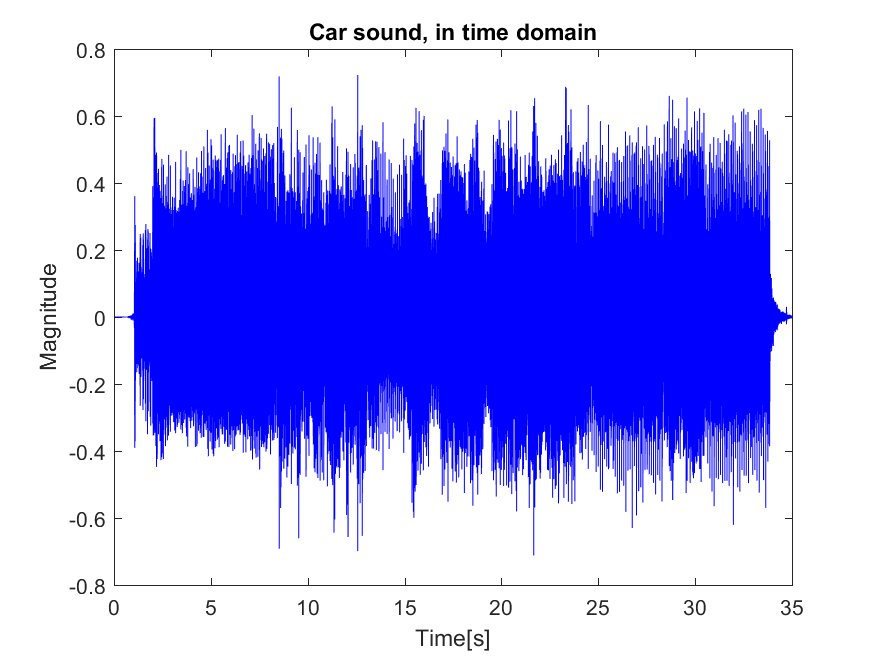
\includegraphics[width=0.45\linewidth]{code/Car_figure1.png}}
	\subcaptionbox{Frequency Domain.\label{fig:car_freq}}
	{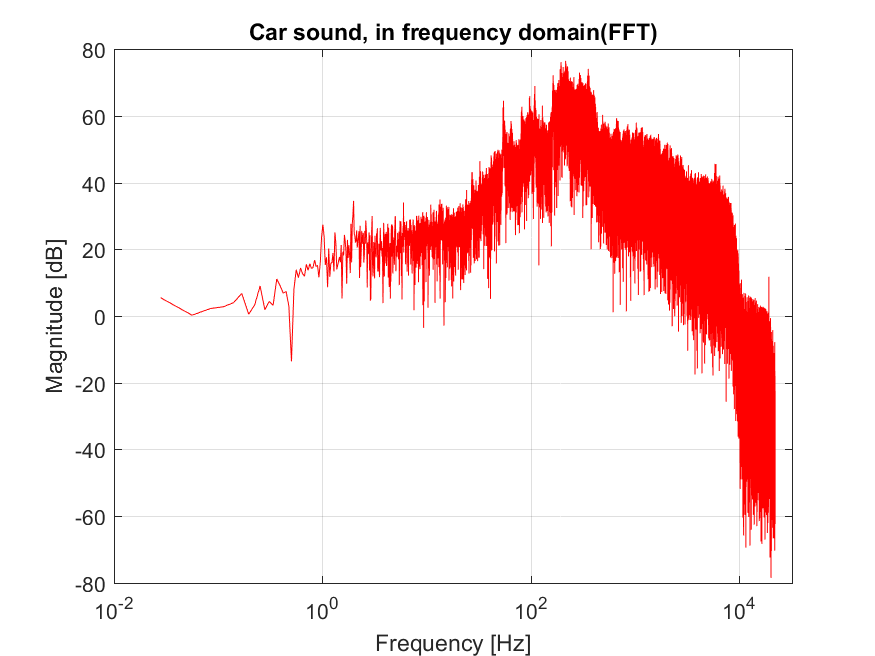
\includegraphics[width=0.45\linewidth]{code/Car_figure2.png}}
	\subcaptionbox{Smoothed fft.\label{fig:car_smooth}}
	{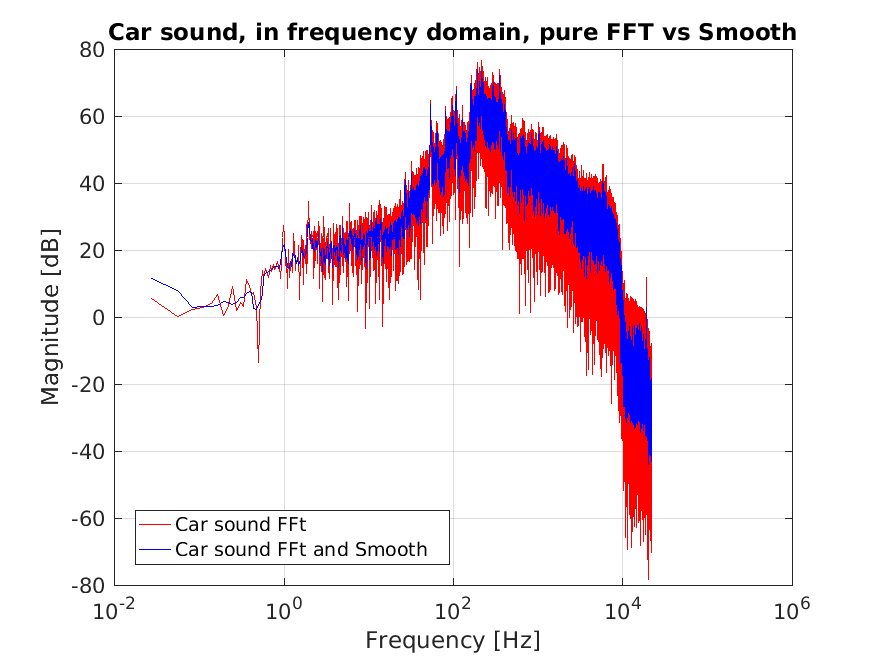
\includegraphics[width=0.45\linewidth]{code/Car_figure3.png}}
	\subcaptionbox{fft of zero padded original.\label{fig:car_zero}}
	{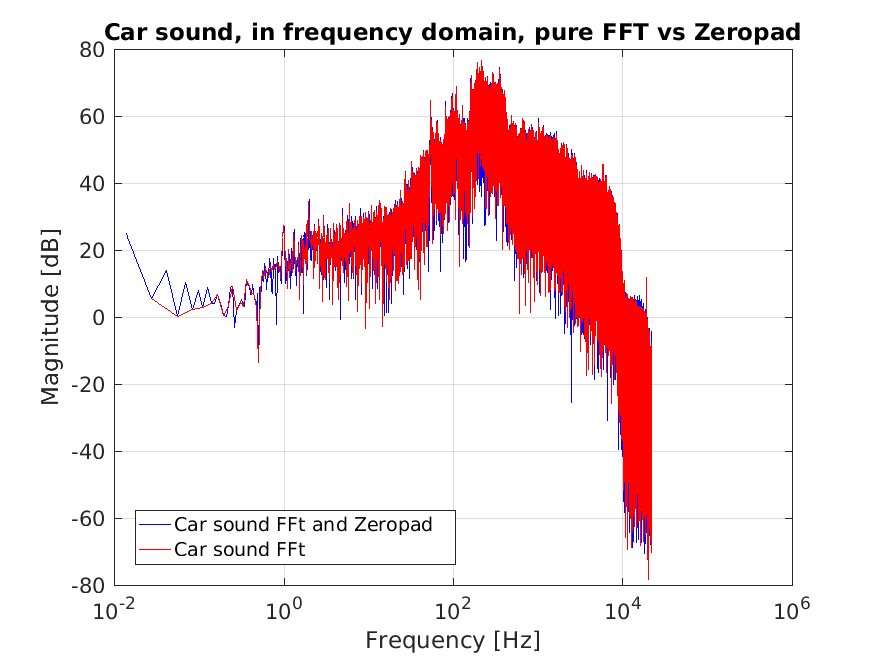
\includegraphics[width=0.45\linewidth]{code/Car_figure4.png}}
	\subcaptionbox{fft of windowed original.\label{fig:car_window}}
	{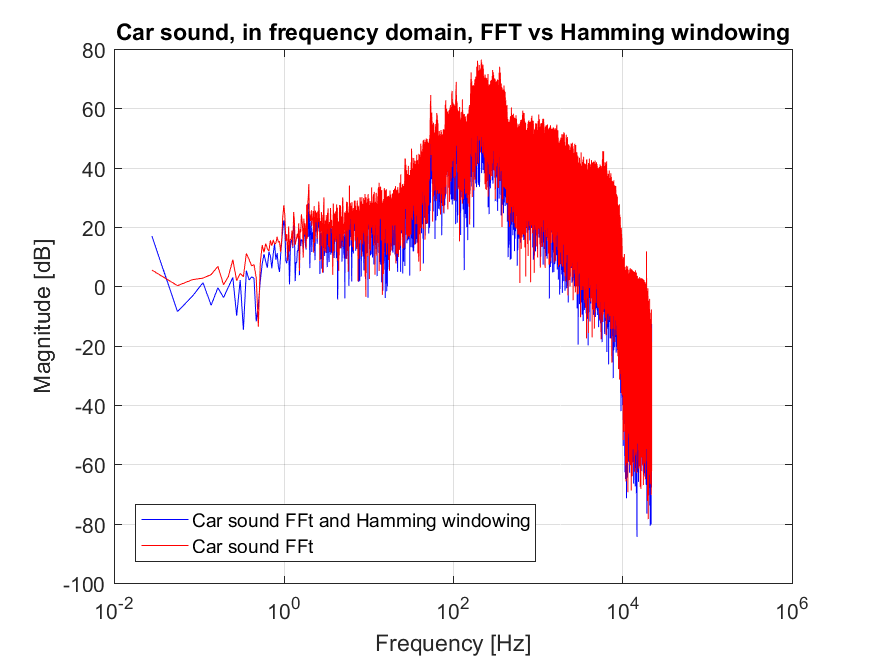
\includegraphics[width=0.45\linewidth]{code/Car_figure5.png}}
	\caption{Analysis of the sound of a car.}\label{fig:car}
\end{figure}

\subsection{Noise from a Windmill}
\begin{figure}[htb]
	\centering
	\subcaptionbox{Time Domain.\label{fig:windmill_time}}
	{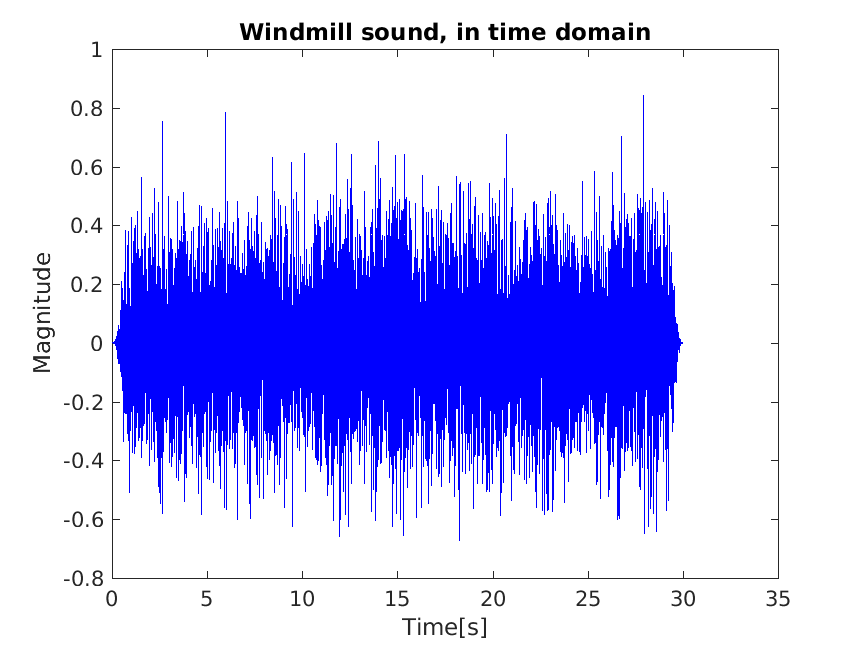
\includegraphics[width=0.45\linewidth]{code/Windmill_figure1.png}}
	\subcaptionbox{Frequency Domain.\label{fig:windmill_freq}}
	{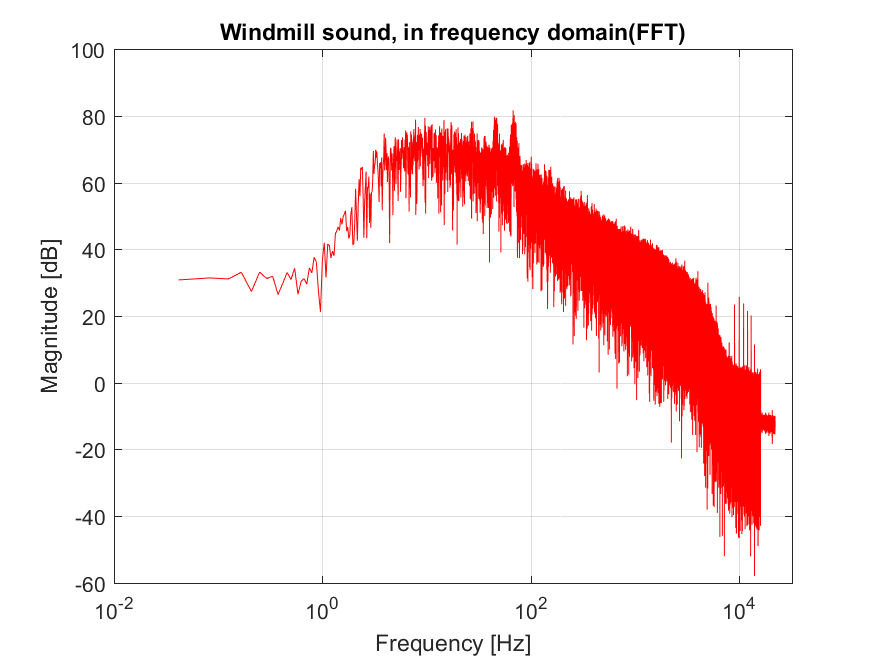
\includegraphics[width=0.45\linewidth]{code/Windmill_figure2.png}}
	\subcaptionbox{Smoothed fft.\label{fig:windmill_smooth}}
	{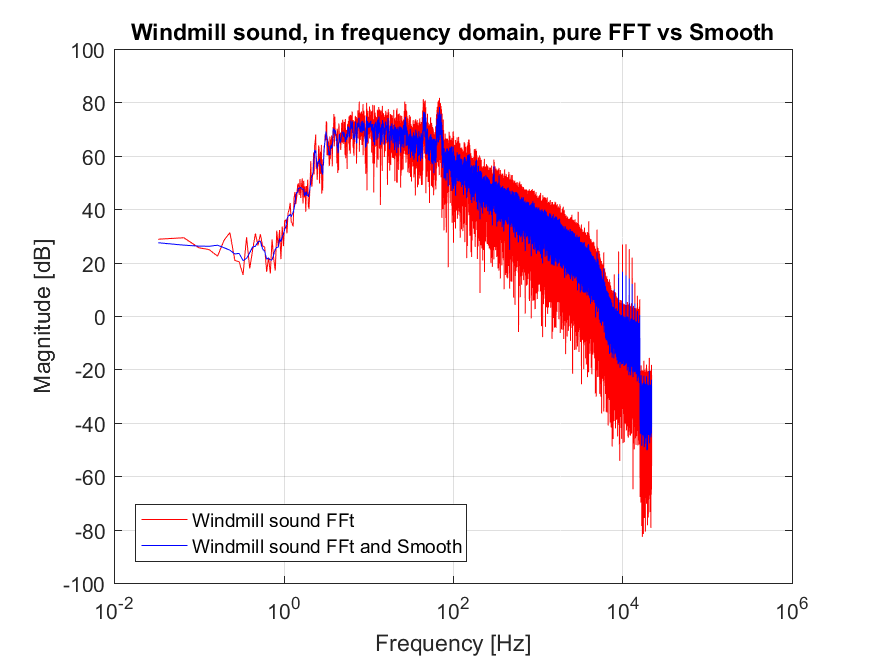
\includegraphics[width=0.45\linewidth]{code/Windmill_figure3.png}}
	\subcaptionbox{fft of zero padded original.\label{fig:windmill_zero}}
	{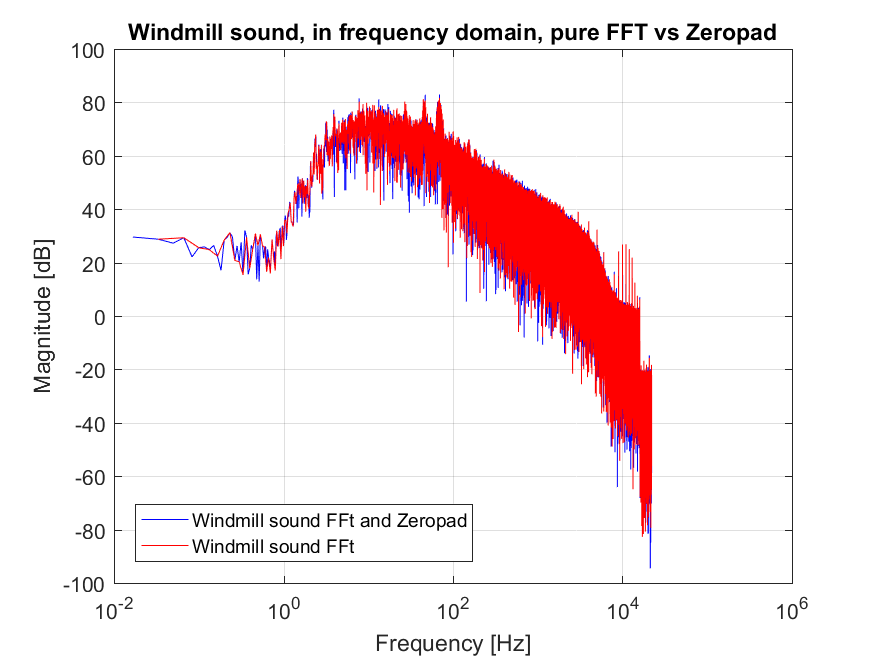
\includegraphics[width=0.45\linewidth]{code/Windmill_figure4.png}}
	\subcaptionbox{fft of windowed original.\label{fig:windmill_window}}
	{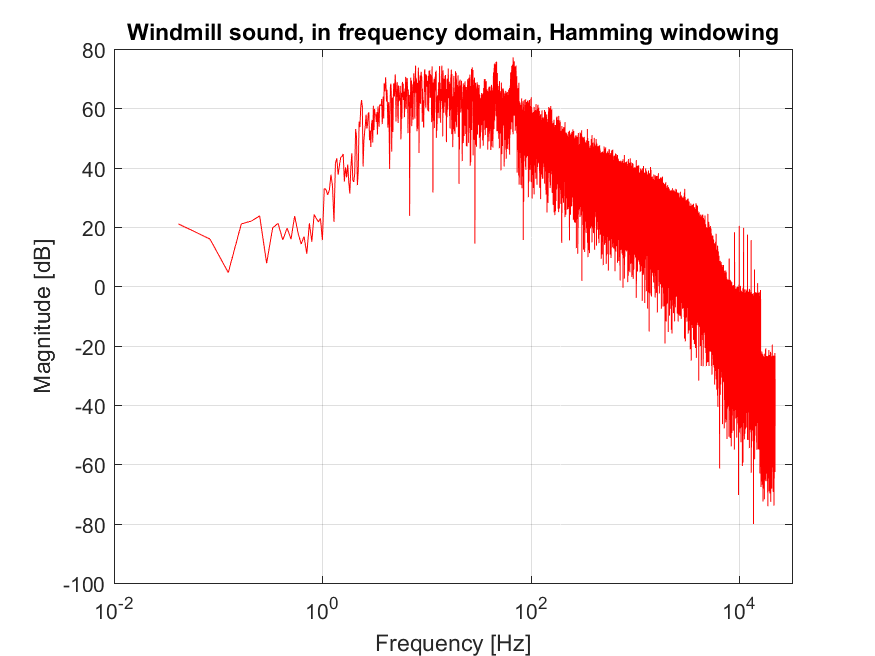
\includegraphics[width=0.45\linewidth]{code/Windmill_figure5.png}}
	\caption{Analysis of the sound of a windmill.}\label{fig:windmill}
\end{figure}


\subsection{EKG}


\subsection{Breaking wine glass}


\subsection{Music}

\paragraph{Genre 1}
Pentatonix (OMI Cover) - Cheerleader

\paragraph{Genre 2}


\paragraph{Genre 3}

\paragraph{Genre 4}

\subsubsection{Conclusion}


\section{Energy} 
\Cref{tab:Energy} shows the energies in signals before and after the Fourier transform. It clearly shows that there is no loss of energy between the original signal and a Fourier transform, but when smoothing and windowing is applied there is a potential loss of energy.
While zero padding does not add or remove any energy from the signal.
\begin{table}[htb]
	\centering
	\begin{tabularx}{\textwidth}{p{2cm} | X X X X X}
		& \rotatebox{90}{\textbf{Time Domain $\times\num{e4}$}}   & \rotatebox{90}{\textbf{Frequency Domain $\times\num{e4}$}} & \rotatebox{90}{\textbf{Smooth $\times\num{e3}$}}     & \rotatebox{90}{\textbf{Zero Padding $\times\num{e4}$}}  & \rotatebox{90}{\textbf{Windowing $\times\num{e4}$}} \\
		\hline
		Car Engine  & \num{3,07}	& \num{3,07}	& \num{0,686}  &	\num{3,07}  & \num{1,34}  \\
		
		Windmill	& \num{4,14}	& \num{4,14}	& \num{0,521} & \num{4,14} & \num{1,79} \\
		
		Breaking Wine Glass & \num{0,0115}	& \num{0,0115}	& \num{0,155}	& \num{0,0115}	& \num{0,000265} \\
		
		EKG & \num{2,05}	& \num{2,05}	& \num{0,626}	& \num{2,05}	& \num{0,729} \\
		
		Cheerleader & \num{13,4}	& \num{13,4}	& \num{1,29}	& \num{13,4}	& \num{7,39}  \\
		
		Roundtable Rival & \num{29,8}	& \num{29,8}	& \num{1,70}	& \num{29,8}	& \num{12,8}  \\
		
		Micheal Jackson \newline Billie Jean & \num{16,3}	& \num{16,3}	& \num{1,73}	& \num{16,3}	& \num{6,86} \\
		
		Violin \newline Let It Go & \num{2,24}	& \num{2,24}	& \num{0,896}	& \num{2,24}	& \num{1,09}
	\end{tabularx}
	
	\caption{Energy of the different signals shown in \si{\joule}.}
	\label{tab:Energy}
\end{table}

Eksperimenter med udglatning, zero-padding og windowing 